\section{Machine learning algoritmes}
\label{chapter:MLA}

\subsection{Inleiding}
In het vorige hoofdstuk hebben we behandeld wat een zelflerend systeem is. In dit hoofdstuk gaan we dieper in op de verschillende soorten zelflerende algoritmes en beantwoorden we de vraag: \textit{Wat zijn voorbeelden van zelflerende algoritmes en hoe werken ze?} We zullen in deze deelvraag naar drie verschillende algoritmes kijken: \textit{Linear Regression, Support vector machines en Artificial Neural Networks.} \cite{SunilRay} 

\subsection{Linear Regression}
Het eerste machine learning algoritme dat we gaan behandelen is \textbf{linear regression}. Dit algoritme wordt gebruikt voor het voorspellen van een y-waarde bij (een) gegeven x-waarde(n). Om linear regression te kunnen gebruiken is het belangrijk dat er wel een lineair verband bestaat tussen de waardes van x en y. In figuur \ref{fig:LinearRegression1} is een dergelijk linear verband te zien. 
Dit lineaire verband is te beschrijven met een formule in de vorm: \textit{y = ax + b}

\begin{figure}[h]
  \centering
    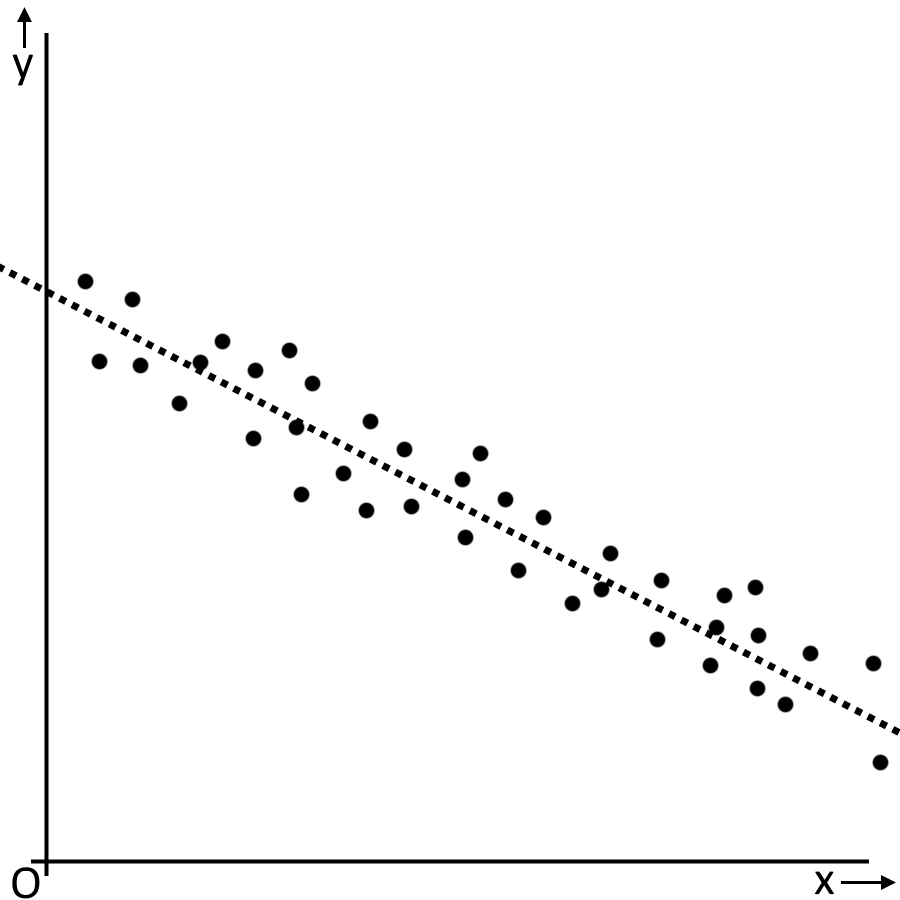
\includegraphics[width=0.5\textwidth]{linearRegression.png}
  \caption{Linear regression}
  \label{fig:LinearRegression1}
\end{figure}

Het doel bij linear regression is het bepalen van de waarde voor a en b in de formule $ y = ax + b $. Dit is op verschillende manieren mogelijk. Een statistische manier hiervoor is door gebruik te maken van het \textbf{ordinary least squares} algoritme. Dit algoritme bepaalt de best passende lijn door de punten, ook wel bekend als de trendlijn. De waarden voor a en b worden hierbij als volgt bepaald:

\begin{align*}
	a&=\frac{\sum_{i=0}^{n}(x_{i}-\bar{x})(y_{i}-\bar{y})}{\sum_{i=0}^{n}{(x_{i}-\bar{x}})^{2}}\\
	b&=\bar{y}-(a * \bar{x})
\end{align*}

In deze formules is $\bar{x}$ het gemiddelde van alle x-waarden en de $\bar{y}$ het gemiddelde van alle y-waarden. 
Dit algoritme is echter alleen toepasbaar als er sprake is van \'{e}\'{e}n x-waarde als invoer, dus geen multidimensionale invoer waarden zoals $(3,3)$. Bij meerdere x-waarden is dit algoritme dus niet te gebruiken. Een andere manier om de a en b waarde te vinden is door gebruik te maken van een leerstrategie. In deelvraag 4 bespreken we drie verschillende leer strategie\"en.

\subsection{Support vector machine}
Een support vector machine (SVM) is een machine learning algoritme ontwikkeld door Vladimir Vapnik \cite{VladimirVapnik}. Het algoritme kan gebruikt worden voor het classificeren van data. Het algoritme is een vorm van supervised learning \cite{SVM}.

\begin{figure}[h]
  \centering
    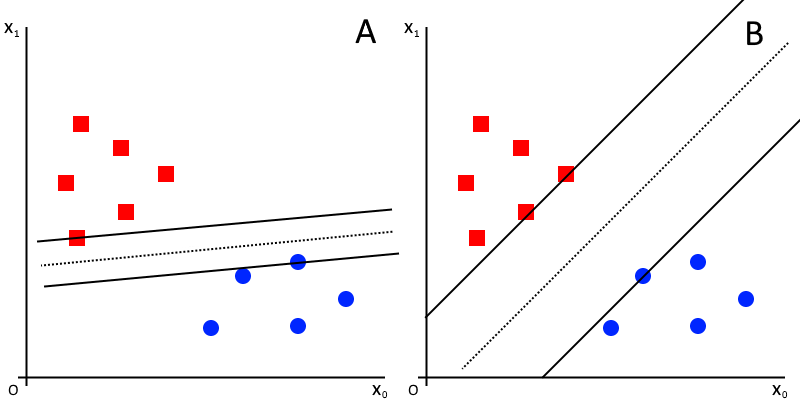
\includegraphics[width=0.5\textwidth]{SVM.png}
  \caption{Support vector machines}
  \label{fig:SupVectorMachine1}
\end{figure}

Een support vector machine werkt als volgt: het trekt een lijn, een \textbf{vector}, tussen twee groepen. Deze vector wordt z\'o getrokken, dat \textit{de afstand tussen de vector en het dichtstbijzijnde datapunt zo groot mogelijk is} \cite{SVM2}. Deze dichtstbijzijnde datapunten worden de \textbf{support vectoren} genoemd. In figuur \ref{fig:SupVectorMachine1} is twee keer dezelfde dataset weergegeven. In de linker afbeelding is te zien dat de vector de twee groepen scheidt maar de afstand tussen het dichtstbijzijnde datapunt kleiner is dan bij de rechter afbeelding, deze afstand wordt de \textbf{marge} genoemd. In de rechter afbeelding is de marge het grootst, dus dit is de betere vector. Het gebied tussen de twee support vectoren wordt de \textbf{hyperplane} genoemd.

\subsubsection{Het agoritme}
Het doel van het algoritme is van een nieuw datapunt bepalen of het tot groep A (de rode vierkantjes) of groep B (de blauwe cirkels) behoort. Als een nieuw datapunt behoort tot groep A dan willen we dat de output van het algoritme negatief is en als het nieuwe datapunt behoort tot groep B willen we dat de output positief is. Hoe positiever of negatiever de output is, hoe zekerder het is dat dit punt daadwerkelijk tot die groep behoort. Als de output 0 is, dan bevindt het punt zich precies tussen de twee groepen, het ligt dan op de stippellijn van figuur \ref{fig:SupVectorMachine1}. Verder is het zo dat de output tussen -1 en 1 ligt als het binnen de twee support vectoren ligt. In dit gebied is het niet helemaal zeker tot welke groep het punt behoort. 
We kunnen de drie vectoren als volgt defini\"eren: 

\begin{center}
De linker support vector	\textit{w * x - b = -1}
\\De middelste vector			\textit{w * x - b = 0}
\\De rechter support vector 	\textit{w * x - b = 1}
\end{center}

Bij het trekken van een lijn probeert een support vector machine het volgende te bereiken:

\begin{itemize}
\item Alle datapunten moeten buiten de twee support vectoren liggen
\item De afstand tussen de support vectoren moet zo groot mogelijk zijn
\end{itemize}


Vanuit de vectoren zijn de volgende twee formules af te leiden:
\begin{itemize}
\item De formule voor of een datapunt buiten de twee support vectoren ligt: $y_{i}(w^{T}x_{i} - b) \geq 0 $
\item De formule voor de afstand tussen de twee support vectoren: $\frac{2}{||w||}$ ($||w||$ betekent de lengte van de vector)
\end{itemize} 


Een vector die voldoet aan de volgende eisen wordt gekozen:
\begin{itemize}
\item Voor alle datapunten moet gelden: $y_{i}(w^{T}x_{i} - b) \geq 0 $
\item $\frac{2}{||w||}$ moet zo klein mogelijk zijn, ofwel $||w||$ zo groot mogelijk
\end{itemize}



\subsubsection{Kernel Methods}
In veel gevallen zal de dataset niet zo mooi geordend zijn als in figuur \ref{fig:SupVectorMachine1}. Het is dan niet mogelijk om een rechte lijn te trekken die de twee groepen scheidt. Een support vector machine zou in dit geval dus niet werken. Om toch een support vector machine te kunnen gebruiken is er een techniek genaamd de \textbf{kernel krick}.

\begin{figure}[H]
  \centering
    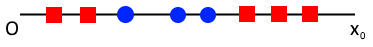
\includegraphics[width=0.5\textwidth]{dataset1d.png}
  \caption{Een \'{e}\'{e}n dimensionale dataset}
  \label{fig:SupVectorMachineKernel}
\end{figure}

In figuur \ref{fig:SupVectorMachineKernel} is een \'{e}\'{e}n dimensionale dataset te zien. Dit wil zeggen dat er maar \'{e}\'{e}n variabele is. Met een support vector machine is het nu niet mogelijk om een lijn te trekken die de twee groepen scheidt. Daarom wordt er een extra variabele bij gemaakt, bijvoorbeeld $X_{1} = (X_{0})^{2}$. Nu is het wel mogelijk een lijn te trekken door de dataset die de twee groepen opdeelt (zie figuur \ref{fig:SupVectorMachine2}). Deze methode kan ook toegepast worden in situaties met meerdere dimensies.

\begin{figure}[H]
  \centering
    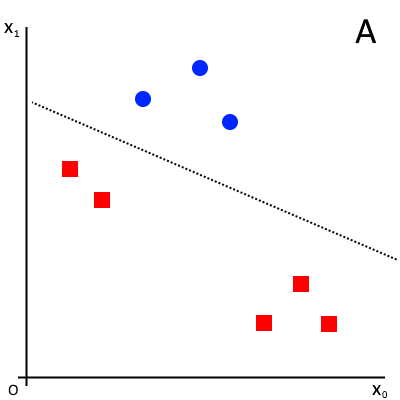
\includegraphics[width=0.5\textwidth]{KernelMethod.png}
  \caption{Een dataset, met een willekeurig uitgevoerde kernel trick}
  \label{fig:SupVectorMachine2}
\end{figure}


\subsection{Artificial Neural Networks}
\subsubsection{Biologisch en kunstmatig netwerk}
Binnen mensen wordt informatie overgebracht door middel van het zenuwstelsel. Dit zenuwstelsel is opgebouwd uit miljarden zenuwcellen. Een zenuwcel, ook wel een neuron genoemd, is opgebouwd uit drie delen: een cel lichaampje, een aantal dendrieten en \'{e}\'{e}n axon. In figuur \ref{fig:BiologischNeuron} is een weergave van een biologische neuron te zien.

\begin{figure}[h]
  \centering
    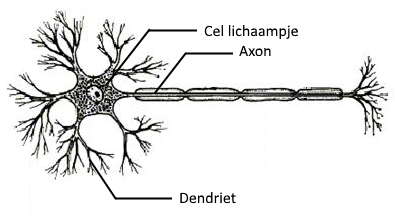
\includegraphics[width=0.5\textwidth]{BiologischNeuron.png}
  \caption{Een tekening van een biologisch neuron}
  \label{fig:BiologischNeuron}
\end{figure}

In de biologie zijn dendrieten verantwoordelijk voor de instroom van informatie. Zij brengen informatie (impulsen) naar het cellichaampje toe. De zenuwcel kan deze informatie vervolgens via een enkele axonen doorgeven aan een dendriet van een andere zenuwcel of aan een spier. Het doorgeven van informatie gebeurt in de uiteindes van de axonen en dendrieten, in zogeheten \textbf{synapsen}.

Het principe van een neuron kan ook door een computer uitgevoerd worden. Dit is het idee voor een Artificial Neural Network (ANN). Een dergelijk netwerk bestaat uit een verschillend aantal ‘computerneuronen’. Elk van deze neuronen krijgt, net zoals een biologische neuron, informatie binnen. Binnen de neuron vindt een berekening plaats. Vervolgens wordt de berekende waarde doorgegeven aan de volgende neuron of gegeven als output.

\subsubsection{De perceptron}
De simpelste vorm van een neural network is een netwerk met slechts \'{e}\'{e}n neuron. Zo'n ANN, voor het eerst gemaakt door  F. Rosenblatt in 1958 \cite{ANN1}, wordt een \textbf{perceptron} genoemd.

\begin{figure}[H]
  \centering
    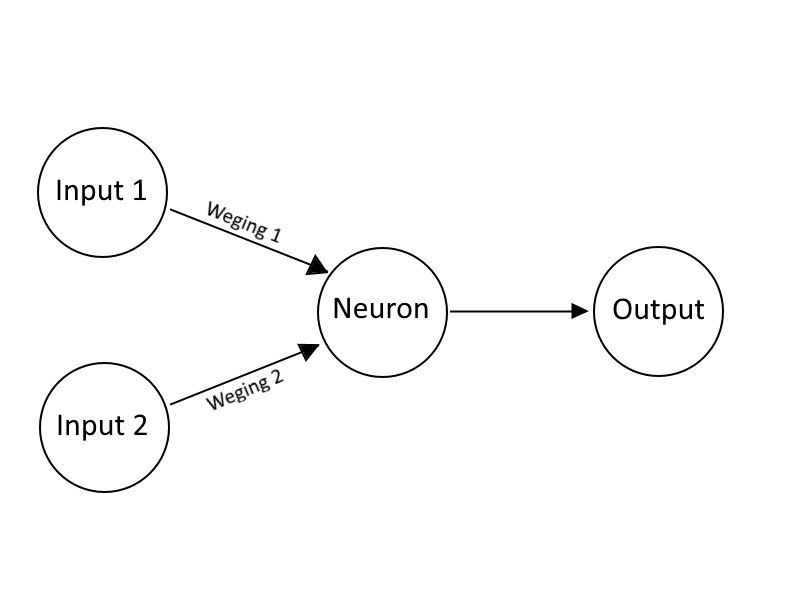
\includegraphics[width=0.5\textwidth]{Perceptron.png}
  \caption{een schematische weergave van en perceptron}
  \label{fig:perceptron}
\end{figure}

In figuur \ref{fig:perceptron} is te zien dat een neuron twee inputs binnen krijgt en daarna een output geeft. De pijlen naar de neuron toe en er vanaf stellen de synapsen voor. Elke synaps heeft een bepaalde weging. De weging van een synaps bepaalt hoeveel invloed die ene input heeft op het netwerk. Het uiteindelijke doel van een neural network is \textit{het zoeken naar de optimale weging voor alle synapsen binnen het netwerk.} 
Om tot een output te kunnen komen moet de neuron een berekening uitvoeren. In deze situatie is de berekening nog vrij eenvoudig:

\begin{center}
$ Som van inputs = X_{1} * W_{1} + X_{2} * W_{2}$
\end{center}

\subsubsection{Activation functions}
De waarde die uit deze berekening volgt, wordt door een \textbf{activation function} gehaald. Een activation function zorgt er voor dat aan deze som een waarde kan worden gehangen, bijvoorbeeld 1 of -1, zonder dat de som absoluut deze waarde heeft. Dit wordt gedaan door te kijken waar het punt op de grafiek van deze functie zich bevind.

\begin{figure}[h]
  \centering
    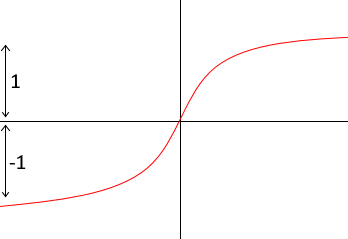
\includegraphics[width=0.5\textwidth]{GenericActivationFunction.png}
  \caption{Een voorbeeld van een algemene activation function en welke waardes hieraan worden gekoppeld.}
  \label{fig:actFunction}
\end{figure}

In figuur \ref{fig:actFunction} is een grafiek van een activation function gegeven. In dit voorbeeld worden aan alle positieve y waardes een 1 verbonden en aan alle negatieve een -1.

Een ANN is een vorm van supervised learning. Het programma weet dus wat het antwoord zou moeten worden. Als de output correct is zal er weinig gebeuren, maar als de output incorrect is zal het programma zichzelf moeten aanpassen om w\'el de goede uitkomst te krijgen. Dit gebeurt met behulp van de wegingen van elke synaps. Deze wegingen kunnen namelijk worden aangepast. De invloed van elke input kan ofwel vergroot ofwel verkleind worden. Op deze manier zal uit de berekening in de neuron de volgende keer misschien een andere, betere uitkomst komen. De nieuwe weging van een synaps wordt nu: $ w_{0} = w_{1} + \Delta w $.
Hoe $ \Delta $w wordt berekend, wordt bepaald door de leerstrategie van het systeem. Hier wordt in het volgende hoofdstuk verder op in gegaan.

\subsubsection{Bias}
Met de besproken perceptron is echter een probleem. Wanneer beide inputs gelijk zijn aan nul heeft het aanpassen van wegingen geen effect. Een weging maal nul zal immers altijd in nul resulteren. Om dit probleem tegen te gaan, wordt er een \textbf{bias} toegevoegd. Dit is een extra input die standaard gelijk is aan \'{e}\'{e}n. De weging van de synaps van de bias wordt niet veranderd. Omdat de neuron nu ook bij inputs van nul een andere uitkomst uit de berekening zal geven, zal er nu toch een getal door de activation function gaan en zullen de wegingen toch worden aangepast. 

\subsubsection{Een netwerk van perceptrons}
Natuurlijk is het ook mogelijk om niet \'{e}\'{e}n, maar meerdere perceptrons te hebben. Zo wordt het een echt netwerk van synapsen en neuronen.

\begin{figure}[h]
  \centering
    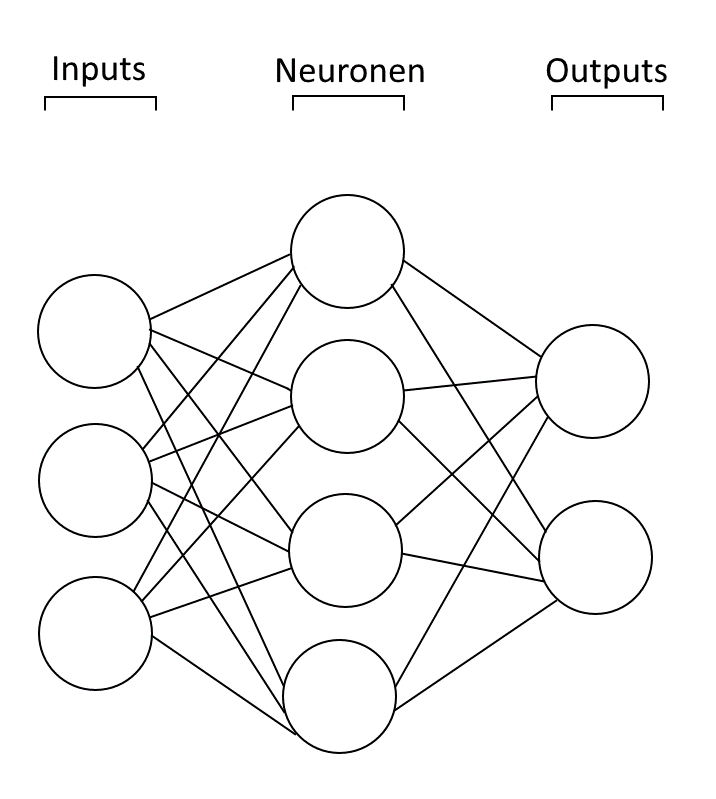
\includegraphics[width=0.5\textwidth]{GenericNeuralNetwork.png}
  \caption{Een schematische weergave van een willekeurig ANN.}
  \label{fig:ANN}
\end{figure}

De laag neuronen noemen we de \textbf{hidden layer}. Het is ook mogelijk meerdere lagen neuronen in de hidden layer te hebben. Dit wordt een \textbf{deep neural network} genoemd, of simpelweg \textbf{deep learning}.
De tot nu toe besproken ANN’s hebben hun informatie allemaal in \'{e}\'{e}n richting bewogen: van alle inputs, naar alle neuronen, naar alle outputs. Dit wordt \textbf{feedforward} genoemd. Ook zou je een neural network kunnen hebben waarin de informatie ook nog tussen de neuronen in dezelfde laag beweegt: een \textbf{recurrent neural network}.

\subsection{Conclusie}
Voorbeelden van zelflerende algoritmes zijn: \textit{Linear regression}, \textit{Support vector machines} en \textit{Arteficial Neural Networks}. Alle drie de algoritmes werken verschillend en zijn goed voor verschillende scenario's. Linear regression werkt door het opstellen van een lineare formule door waarden met een linear verband. Support vector machines werken door een vector te maken die twee groepen zo goed mogelijk scheidt. En Arteficial neural networks werken door een netwerk van neuronen te simuleren.
